\chapter{Handleiding desktop applicatie}

De desktopapplicatie bevindt zich op de computer 'Nernst'.
Op deze machine kan je inloggen met de gebruikersnaam 'Administrator' en het bekende wachtwoord 'e=mc**2'.
De desktopapplicatie bevindt zich in de map 'VOP Groep 7' op het bureaublad en kan je opstarten doormiddel van de snelkoppeling 'StockPlay administratie'.

\section{Algemene zaken}

Inloggen:
De inloggegevens voor deze demo zijn "Administrator" en "chocolademousse". Je kan ook zelf een account aanmaken in gebruikersbeheer. Als deze de rechten 'Administrator' bezit, dan kan je hiermee ook inloggen.

\begin{figure}[h!]
	\centering
		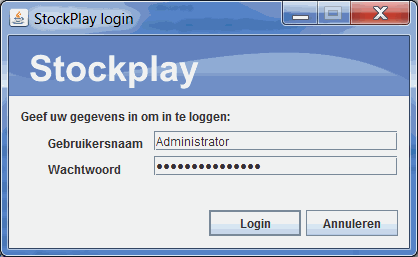
\includegraphics[width=\textwidth]{images/handleiding/handleiding1.png}
	\caption{Inlogformulier}
\end{figure}

Het standaard openingsscherm bevat een overzicht van de status van de verschillende componenten.
Alsook bevat deze enkele belangrijke statistieken:
Op het moment van schrijven is de logica in de 'backend' die achter de Start/Stop/Restart-knoppen zit nog niet uitgewerkt.

\begin{figure}[h!]
	\centering
		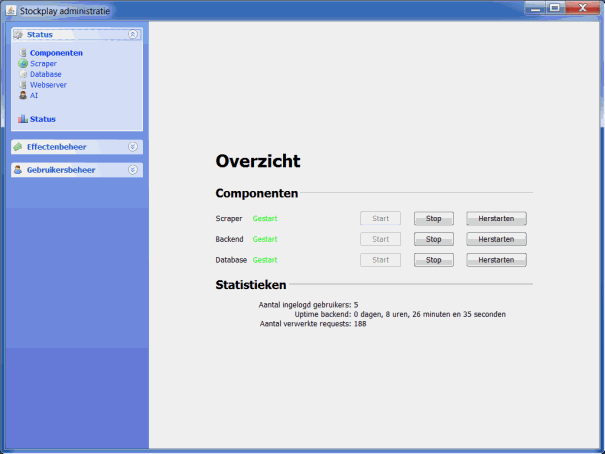
\includegraphics[width=\textwidth]{images/handleiding/handleiding7.png}
	\caption{Overzicht van de componenten}
\end{figure}

\section{Beheer van effecten}

Als je op "Effectenbeheer" in de linkerkolom klikt verschijnt onderstaand scherm (het inladen van de effecten duurt een kan even duren).
In het uitschuifmenu bevinden zich enkele filters die je kan activeren door ze aan te klikken.

\begin{figure}[h!]
	\centering
		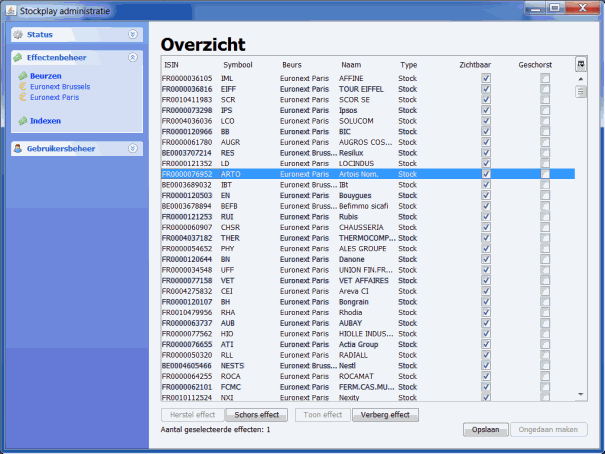
\includegraphics[width=\textwidth]{images/handleiding/handleiding6.png}
	\caption{Overzichtscherm voor het effectenbeheer}
\end{figure}

Op elk effect kan je de volgende acties uitvoeren:

\begin{itemize}
\item{Naam wijzigen (in de tabel klikken)}
\item{Type wijzigen (in de tabel klikken)}
\item{Zichtbaarheid wijzigen (in de tabel klikken, of de effecten selecteren en de knoppen onderaan gebruiken)}
\item{Geschorst-zijn wijzigen (in de tabel klikken, of de effecten selecteren en de knoppen onderaan gebruiken)}
\end{itemize}

Om de wijzigingen permanent te maken klik je vervolgens op de knop "Opslaan".

\section{Beheer van gebruikers}

Als je "Gebruikersbeheer" in het navigatiemenu aanklikt, verschijnt het gebruikersbeheer..
Links verschijnt er ook terug een aantal filters die je kan activeren.

\begin{figure}[h!]
	\centering
		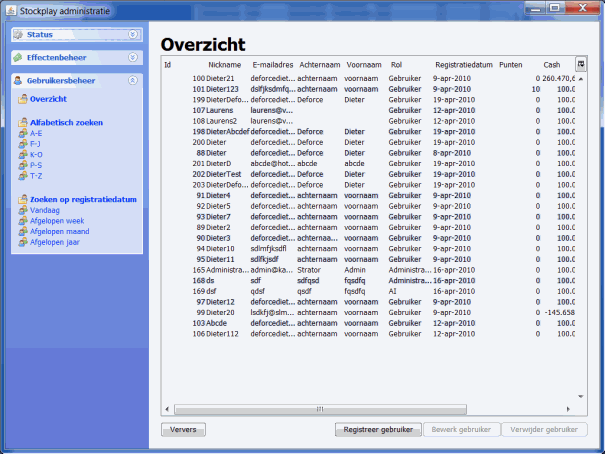
\includegraphics[width=\textwidth]{images/handleiding/handleiding5.png}
	\caption{Gebruikersbeheer}
\end{figure}

Opmerking: In tegenstelling tot de wijzingen die je uitgevoerd hebt bij het effectenbeheer zijn alle acties hier direct definitief!!

De mogelijk acties zijn:
\begin{itemize}
\item{Aanmaken van een nieuwe gebruiker met 'Registreer gebruiker'.}
\end{itemize}

\begin{figure}[h!]
	\centering
		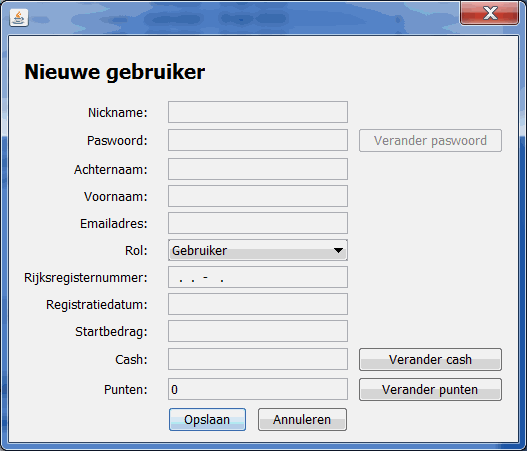
\includegraphics[width=\textwidth]{images/handleiding/handleiding4.png}
	\caption{Een nieuwe gebruiker aanmaken}
\end{figure}

Om een nieuwe gebruiker te registeren moet je de velden Nickname, Paswoord, Achternaam, Voornaam en Emailadres invullen. 
De velden startbedrag, cash en punten worden bij het registeren van de gebruiker in de backend automatisch voor je ingevuld.

Bij het bewerken van een gebruiker verschijnt een gelijkaardig venster als dat van "Registreer gebruiker".
Dit venster verschilt hierin in de volgende punten:

\begin{itemize}
\item{Om het wachtwoord te veranderen, klik je op de knop "Verander paswoord", vervolgens verschijnt het wachtwoord veld}
\item{De hoeveelheid cash en punten kan worden gewijzigd. De applicatie vereist echter wel dat dit gelogged wordt, en daarom verschijnt er een nieuw scherm waar je een reden dient op te geven..}
\end{itemize}

\begin{figure}[h!]
	\centering
		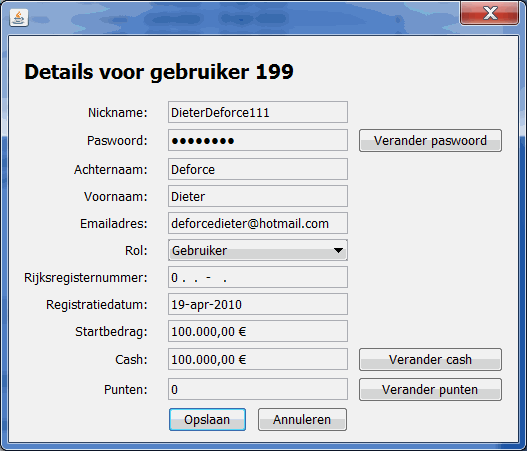
\includegraphics[width=\textwidth]{images/handleiding/handleiding3.png}
	\caption{Details voor een gebruiker bekijken}
\end{figure}

\begin{figure}[h!]
	\centering
		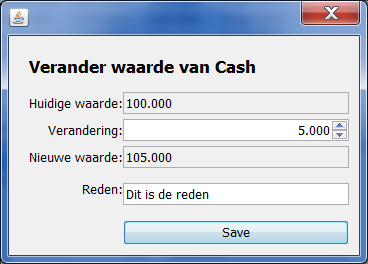
\includegraphics[width=\textwidth]{images/handleiding/handleiding2.png}
	\caption{Een wijziging in de cashpositie van een gebruiker vastleggen.}
\end{figure}

\chapter{Handleiding webapplicatie}

De website is te bereiken op het interne schoolnetwerk op het internetadres 'http://nernst/'.
Buiten het schoolnetwerk kan men een versie van de site bekijken op 'http://www.kapti.com'.

De welkomstpagina verschijnt waarin een korte omschrijving van het spel gegeven wordt. Het navigatiemenu links op de pagina en het informatieblok onderaan worden op elke pagina weergegeven. In dat informatieblok kan je informatie vinden over het pad van de huidige pagina die je bekijkt. De aangemelde gebruiker staat ook in het informatieblok. Als je naar deze overzichtspagina terug wil keren kan je het item 'Home' aanklikken in het navigatiemenu.

Klik je in het navigatiemenu de optie Ranking aan, dan krijg je een overzicht te zien van de tien spelers die op dit moment de hoogste score behaald hebben.
Deze pagina is op het moment van schrijven nog niet afgewerkt.

Je kan de pagina "Help" aanklikken om een nog wat extra algemene informatie over het spel en ook de status van het project te bekijken.

De pagina's 'Portfolio', 'Orders' en 'Transaction History' werken enkel maar als een gebruiker aangemeld is.
Om te kunnen aanmelden dien je eerst over een lidmaatschap te beschikken. Een lidmaatschap kan je verkrijgen door in het informatieblok op de verwijzing 'Register' te klikken. Je kan vervolgens een gebruikersnaam kiezen en een wachtwoord opgeven. Na het invullen van de velden klik je 'Regsitreer' aan.
Na het doorlopen van deze procedure zal je ook een email ontvangen hebben. Die kan je bewaren ter geheugensteuntje voor je gebruikersnaam.
Nu heb je een persoonlijk lidmaatschap. Om het te activeren kan je inloggen met de gekozen gebruikersnaam en bijhorende wachtwoord.

\section{Overzicht van effecten - opvragen van details}

Onder "Securities Overview" krijg je een overzicht te zien van de effecten die op dit moment in het StockPlay systeem aanwezig zijn. Je kan in het navigatiemenu ook rechtstreeks een beurs aanklikken. Zo krijg je al direct een eerste filtering op de lijst.
Op dit moment gebeurd het ophalen nog wat traag. Dit komt omdat door de abstractielagen nogal wat verbindingen tussen verschillende lagen en servers opgezet moeten worden.
De beurzen onder "Securities Overview" zijn die die op dit moment in het spel aanwezig zijn en waarop gescrapped wordt.

Klik je op de naam van een effect, dan krijg je detailinformatie te zien over een effect.
Je vind er de huidige prijs, verandering, de beurs waar deze op noteert, de ISIN code, het symbool, de openingsprijs, de maximumprijs van die dag en de laagste prijs van de laagste verhandelingsdag.

De grafiek kent vele mogelijkheden.
Deze is opgebouwd uit twee delen. Het bovenste deel bevat een weergave van het prijsverloop van het gekozen effect. Onderaan zijn bargrafieken te zien van de volumes. Het bovendeel toont standaard het verloop van de voorbije 7 dagen. Hierop kunnen een aantal handelingen verricht worden.
Als je de muisaanwijzer boven dit deel gaat hangen verschijnt het menu.

Met de selectie knop wijzig je de modus van de muis. Standaard staat deze op de verplaats modus.
In deze modus kan je dubbel klikken op een locatie om daarop in te zoomen. Of je kan meer detail krijgen door met de muisaanwijzer het deel aan te wijzen waar je meer detail op wil en het muiswieltje naar boven te verplaatsen. Verplaats het wieltje naar onderen om terug uit te zoomen.
Je kan ook een deel van de grafiek aanklikken en verslepen. Het tekengebied wordt pas opnieuw getekent nadat de linker muisknop losgelaten is.
In de selectie modus is het nog steeds mogelijk om meer of minder detail te verkrijgen door dubbel te klikken en het scrolwieltje te gebruiken.
Alleen ga je in deze modus bij het slepen niet de grafiek verplaatsen, maar een detail venster aanduiden dat je wil bekijken.

Gebruik de knop 'vorige' om het vorige beeld terug op te roepen. Deze knop kan je oneindig blijven gebruiken tot je terug in de standaardweergave terechtkomt.

Met de knoppen 'kleiner' en 'groter' is het opnieuw mogelijk om meer of minder detail op te vragen.

Klik op 'Toevoegen' om een referentie toe te voegen. Op het huidige moment is dit nog een vaste referentie, maar in de toekomst zal het mogelijk zijn deze zelf te kiezen. Een extra lijn wordt bijgetekend. Deze kan je weghalen door in de legende de x aan te klikken rechts van de referentie die je wenst te verwijderen.
Het zal in de toekomst ook mogelijk zijn meerdere referenties toe te voegen.

De 'Herstel' actie gaat de standaardweergave van de grafiek herstellen. Referenties en weergave geschiedenissen worden terug weggehaald.

Alle datapunten in de grafiek worden dynamisch opgehaald via AJAX technologie na het wijzigen van de view. Het kan dus even duren voor de nieuwe wijzigen zichtbaar worden. Bij het uitzoomen worden minder punten en dus minder detail opgehaald. Het zal nooit mogelijk zijn een tijdsdeel te bekijken waar geen data voor handen is voor ofwel de hoofdgrafiek ofwel voor de referentielijnen. Het maximum uitgezoomde level toont dus alle data die momenteel in het systeem zit.

'Portfolio', 'Orders' en 'Transaction History' bieden overzichten voor de huidige ingelogde gebruiker.

\section{Aankopen van effecten}

Klik links op "Securities Overview" of een van de beurzen die aanwezig is in het spel om een lijst te krijgen van effecten. Klik op de "Buy" knop van het gewenste aandeel. Deze knop is ook te vinden op een detailpagina van een effect.

Je kan een prijs een een aantal aandelen opgeven die je wenst te kopen. Als aan de voorwaarden vervolgens voldaan wordt, dan zal de transactionmanager deze op bepaalde tijdstippen omzetten naar een geldige transactie. Hierbij zal het order dan uitgevoerd worden en worden de effecten aan het portfolio toegevoegd.